\documentclass[11pt]{article}


\usepackage[utf8]{inputenc}
\usepackage[margin=1in]{geometry}
\usepackage{amsmath}
\usepackage{amssymb}
\usepackage{amsthm}
\usepackage{enumerate}
\usepackage{enumitem}
\usepackage{graphicx}
\usepackage{url}
\usepackage{hyperref}
\usepackage{tikz}
\usetikzlibrary{positioning, arrows.meta}


\setlength{\parindent}{0pt}
\hyphenpenalty=10000
\exhyphenpenalty=10000

\begin{document}

\begin{center}
{\Large TODO: Project Title}

\medbreak
{\Large Project Proposal}

\medbreak
{\large ECS240 - Fall 2026}

\medbreak
{\large Prom TODO, Qingze He, Jim Brower}
\end{center}
\vspace{1em}

\begin{enumerate}

%%%%%%%%%%%%%%%%%%%%%%%%%%%%%%%%%%%%%%%%%%%%%%%%%%
%%%%%   Introduction and motivation          %%%%%
%%%%%%%%%%%%%%%%%%%%%%%%%%%%%%%%%%%%%%%%%%%%%%%%%%

\item
\textbf{Introduction and motivation}

\begin{enumerate}[label*=\arabic*.]

\item
\textbf{Problem domain and motivation.}
% Application domain, problem being solved, why it is interesting.
% At least 3 citations, at least 2 research papers.

\item
\textbf{Proposed language.}
% Own toy language, or a subset of an existing language?
% What it contains / what subset of features. Example syntax.

\begin{verbatim}
-- example program
\end{verbatim}

\item
\textbf{Proposed tool.}
% Basic interpreter + one of: compiler, static analysis, dynamic analysis, type system.
% Input/output of the tool. How a user interacts with it.

\item
\textbf{Scope and related work.}
% Is the solution already known/built? Existing tools for similar problems.

\end{enumerate}

\bigbreak

%%%%%%%%%%%%%%%%%%%%%
%%%%%   Goals   %%%%%
%%%%%%%%%%%%%%%%%%%%%

\item
\textbf{Goals}

% High-level goals, described in more detail in later sections.

\medbreak
\textbf{Minimum goal:}
\newline

\medbreak
\textbf{Target goal:}
\newline

\medbreak
\textbf{Reach goal:}
\newline

\bigbreak

%%%%%%%%%%%%%%%%%%%%%%%%%%%%%%%%%%%%%%%%%%%%%%%%%%
%%%%%   Theory part: Syntax and Semantics    %%%%%
%%%%%%%%%%%%%%%%%%%%%%%%%%%%%%%%%%%%%%%%%%%%%%%%%%

\item
\textbf{Theory: Syntax and Semantics}

Our language enables multiple processes to communicate through message queues and provides serialization and deserialization operations. To be more specific, process A receives the initial input. It serializes the input and sends the serialized data to B. After process B receives it, the data will be deserialized. Then, B will print out the original information.


\begin{verbatim}
process A {
    let msg = serialize(input);
    send(B, msg);
}

process B {
    receive(msg);
    print(deserialize(msg));
}
\end{verbatim}

We have string literal $s$, variables $x$ and $y$, and process name $p$. Then, we have $e$ for expressions,
$S$ for statements, $T$ for processes, and $P$ for programs. The variable \texttt{input} is bound to the process's
initial data from INPUT. The expression \texttt{info(e, e)} builds a message with two parts, and
\texttt{receiveinfo(x, y)} receives such a message and binds its two parts to $x$ and $y$.

\begin{verbatim}
e ::= s | x | info(e, e) | serialize(e) | deserialize(e)

S ::= let(x, e)
    | send(p, e)
    | receive(x)
    | receiveinfo(x, y)
    | print(e)
    | seq(S, S)

T ::= process(p, S)

P ::= T | pair(P, P)
\end{verbatim}



We have (INPUT, prog, OUTPUT). INPUT contains the initial data for each process, prog is the program, and OUTPUT is the sequence of printed values. Each process only needs to execute its own statements in sequence, without waiting for other processes to finish. For example, \texttt{send} adds the message to the end of the receiver's queue. The sender does not need to wait for a reply from the receiver. \texttt{receive} takes messages from the queue in first in, first out order. For valid messages, serialization and deserialization satisfy deserialize(serialize(m)) = m. Therefore, the above program outputs [m] when A receives the input m.

\bigbreak

%%%%%%%%%%%%%%%%%%%%%%%%%%%%%%%%%%%
%%%%%   Implementation plan   %%%%%
%%%%%%%%%%%%%%%%%%%%%%%%%%%%%%%%%%%

\item
\textbf{Implementation plan}

\begin{enumerate}[label*=\arabic*.]

\item
\textbf{Tool and language selection.}

We'll be writing everything in Rust, set up as a single Cargo workspace. Our compiler will also target Rust: it turns a program in our language into Rust source, which gets built with
\texttt{cargo} and linked against a runtime library that we write ourselves. Using Rust for both the tools and the runtime means
we can share the AST and value types between components, and the generated code can call straight into the runtime.

\item
\textbf{Incorporating existing tools.}

Mostly from scratch. The instructor said it's fine to use an existing lexer and parser generator, so we plan to use
LALRPOP\cite{lalrpop}, which is the most common parser generator in the Rust ecosystem.

\medbreak
Beyond that, we'd like to stick to the Rust standard library. Message passing is the core feature of our language,
so we don't want to use an existing actor or channel crate to do it for us. Mailboxes will be built from
\texttt{std::sync} primitives, serialization will be our own code, and if we get to communication between OS
processes or machines we'll use \texttt{std::net}.

\item
\textbf{Architecture of your code.}

Our planned architecture is shown below:

\begin{figure}[ht]
  \centering
  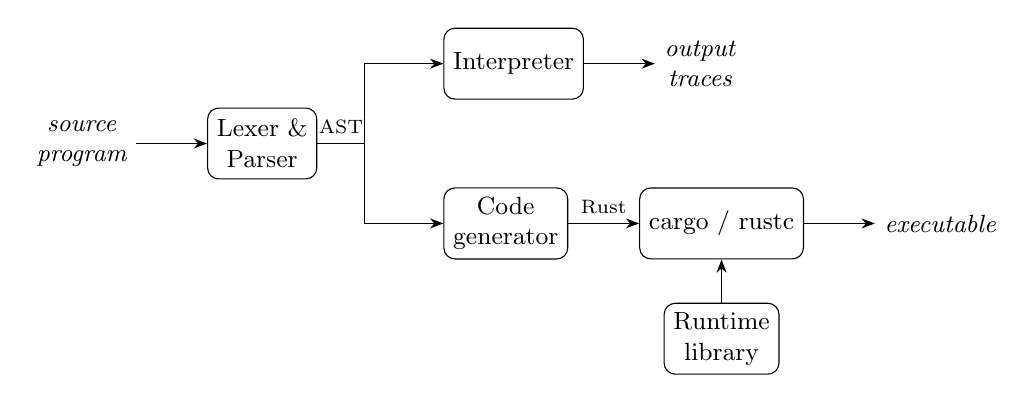
\begin{tikzpicture}[
      node distance=0.55cm and 0.9cm,
      box/.style={draw, rounded corners, align=center, minimum height=0.9cm, font=\small},
      data/.style={align=center, font=\small\itshape},
      arr/.style={-Stealth}
    ]
    \node[data] (src) {source\\program};
    \node[box, right=of src] (parse) {Lexer \&\\Parser};
    \node[box, above right=0.1cm and 1.6cm of parse] (interp) {Interpreter};
    \node[box, below right=0.1cm and 1.6cm of parse] (gen) {Code\\generator};
    \node[data, right=of interp] (traces) {output\\traces};
    \node[box, right=of gen] (cargo) {cargo / rustc};
    \node[box, below=of cargo] (rt) {Runtime\\library};
    \node[data, right=of cargo] (exe) {executable};

    \draw[arr] (src) -- (parse);
    \coordinate[right=0.6cm of parse] (fork);
    \draw (parse) -- node[above, font=\scriptsize] {AST} (fork);
    \draw[arr] (fork) |- (interp);
    \draw[arr] (fork) |- (gen);
    \draw[arr] (interp) -- (traces);
    \draw[arr] (gen) -- node[above, font=\scriptsize] {Rust} (cargo);
    \draw[arr] (rt) -- (cargo);
    \draw[arr] (cargo) -- (exe);
  \end{tikzpicture}
  \caption{Planned architecture.}
  \label{fig:architecture}
\end{figure}

\medbreak
Both the interpreter and the compiler share a front end, which parses the program into an AST following the grammar
in Section 3.

\medbreak
The interpreter is meant to be a direct implementation of the semantics. It runs every process in a single thread
and keeps track of each process's remaining statements, its variables, and its message queue. A scheduler picks
which process takes the next step. We'd like to support a few schedulers: round-robin, random with a seed, and for
small programs, trying every interleaving to get the full set of possible outputs. Since the interpreter sees
everything at once, it can also tell us when the program deadlocks.

\medbreak
The compiler turns each \texttt{process} into a Rust function, with \texttt{send}, \texttt{receive},
\texttt{serialize} and \texttt{deserialize} becoming calls into the runtime. The runtime runs each process on its
own thread and keeps a mailbox for each one (a queue behind a mutex, with a condition variable so \texttt{receive}
can sleep until something arrives). We'll hide message delivery behind an interface, so we can start with everything
in memory and later swap in a version that sends messages between OS processes over TCP.

\item
\textbf{Development effort.}

Looking at Figure~\ref{fig:architecture}, we need to write the grammar and AST, the interpreter
and its schedulers, the runtime, the code generator, and a small command line tool that either runs a program with
the interpreter or compiles it. We'll also need a set of example programs to test with. Since our programs are
nondeterministic, we can't just compare a compiled program against one expected output. Our plan is to run compiled
programs many times and check that every output they produce is one of the outputs the interpreter says is possible.

\medbreak
We will compile directly from the AST at first. If time permits, we'd like to add a small IR and a couple of
simple optimizations such as constant folding.

\medbreak
We are not planning to handle crashed processes or lost messages, or encrypt messages (if
that's ever needed it belongs at the network layer, like TLS). Anything not in the grammar from Section 3, such as
creating new processes at run time, is also out of scope for now.

\item
\textbf{Challenges.}

The biggest challenge is probably nondeterminism. The same program can behave differently from run to run, which
makes bugs hard to reproduce. That's a big part of why we want the interpreter to have seeded and exhaustive
schedulers. A related issue is that a compiled program that deadlocks will just hang. We can try to detect this in
the runtime, but if that gets complicated we'll fall back to a timeout in our tests.

\medbreak
We're also expecting some friction generating Rust code that the Rust compiler accepts, mostly because of ownership
rules. We plan to keep the generated code simple (cloning values where needed) rather than efficient. If LALRPOP
ends up being a poor fit, our grammar is small enough that we could write a recursive descent parser by hand. The
syntax in Section 3 is still a draft, so we'll try to keep changes contained to the parser and the AST. Finally,
networking adds a lot of new problems (finding other processes, connecting, partial failures), so we'll only
attempt it once the in-memory version works.

\end{enumerate}

\bigbreak

%%%%%%%%%%%%%%%%%%%%%%%%%%%%%%%%%%
%%%%%   Collaboration plan   %%%%%
%%%%%%%%%%%%%%%%%%%%%%%%%%%%%%%%%%

\item
\textbf{Collaboration plan}

% How components are divided among team members.

% Group meetings (at least twice a week suggested) and communication platform.

\medbreak
\textbf{Timeline:}

\medbreak
Week of Nov 16:
\newline

\medbreak
Week of Nov 23:
\newline

\medbreak
Week of Nov 30:
\newline

\medbreak
Week of Dec 7:
\newline

\medbreak
\textbf{Commitment statement:}

\medbreak
I commit to work and contribute equally to this project. \hfill --- Prom TODO

\medbreak
I commit to work and contribute equally to this project. \hfill --- Qingze He

\medbreak
I commit to work and contribute equally to this project. \hfill --- Jim Brower

\bigbreak

%%%%%%%%%%%%%%%%%%%%%%%%%%%%%%%%%%%%%%%%%%%%%%%%%%%%%%
%%%%%   Conclusion and questions for feedback   %%%%%
%%%%%%%%%%%%%%%%%%%%%%%%%%%%%%%%%%%%%%%%%%%%%%%%%%%%%%

\item
\textbf{Conclusion and questions for feedback}

% What happens if the project is successful? Why is it exciting/important?

% Open questions and things to get feedback on.

%%%%%%%%%%%%%%%%%%%%%%%%%%%%%%%%
%%%%%   References cited   %%%%%
%%%%%%%%%%%%%%%%%%%%%%%%%%%%%%%%

\end{enumerate}

\bibliographystyle{unsrt}
\bibliography{references}



\end{document}
